\chapter{Attacks}
\label{chapter:attacks}
Various attacks has been performed against Bitcoin in the past.
Attacks can be performed at different levels with very different approaches and can have a wide range of effects on Bitcoin users.
This chapter starts from an overview of the most relevant ones.
At the end, it describes in details the Balance attack, whose analysis is the main object of the simulations.

\section{Double Spending}
Double-spending is the result of successfully spending some money more than once.
The attack is the oldest known one against Bitcoin and it is even partially discussed in the original Bitcoin paper \cite{bitcoin_2009}.
The attack works by creating \num{2} conflicting transactions (that spend all the bitcoins in the same address) and submitting them to different parties, for example \texttt{tx-1} to a merchant and \texttt{tx-2} to the Bitcoin network:
if the merchant accepts \texttt{tx-1} but the Bitcoin network receives \texttt{tx-2} before \texttt{tx-1}, it is likely that \texttt{tx-2} will be stored in the blockchain, while \texttt{tx-1} will be discarded, since not compatible with \texttt{tx-2}.
The attacker only pretends to spend some bitcoins to pay the merchant, but it actually does not spend anything:
it gets the purchase for free, while the merchant never receives the due bitcoins.

Double-spending breaks the most important guarantee that Bitcoin tries to give:
transactions are irreversible and bitcoins can be spent only once.
The double-spending attack can be performed directly in some cases, or can be the result of more complex attacks.
There are many variants of double-spending, we analyze the most common ones here.

\subsection{Race Attack}
The race attack involves merchants that immediately accepts payments, without waiting for the unconfirmed transaction to be securely store in some block in the blockchain \cite{bitcoin_wiki_irreversible_transactions}.
The race attack has a high degree of success for an attacker \cite{double_spending_two_for_one}.
The attack is illustrated in \cref{fig:race-attack} and works as follows:
\begin{itemize}
	\item the attacker sends a transaction \texttt{tx-1} to the merchants;
	\item at the same time, the attacker sends a conflicting transaction \texttt{tx-2} to some miner; the conflicting transaction spend the bitcoins stored in the same address used in \texttt{tx-1} and sends them to new address in control of the attacker;
	\item the merchants sees the unconfirmed transaction and accepts the payment; this scenario is more likely for in-shop purchases, where, in many cases, the merchant can not wait for the transaction to be stored in the blockchain;
	\item \texttt{tx-2} is received before \texttt{tx-1} from the miners, so it is more likely to be stored in some block before \texttt{tx-1};
	\item \texttt{tx-2} is stored in a block, while \texttt{tx-1} is rejected since in conflict with \texttt{tx-1};
	\item the attacker receives its bitcoins back, while the merchant does not get anything.
\end{itemize}

\begin{figure}[h]
	\centering
	\vspace*{0.20cm}
	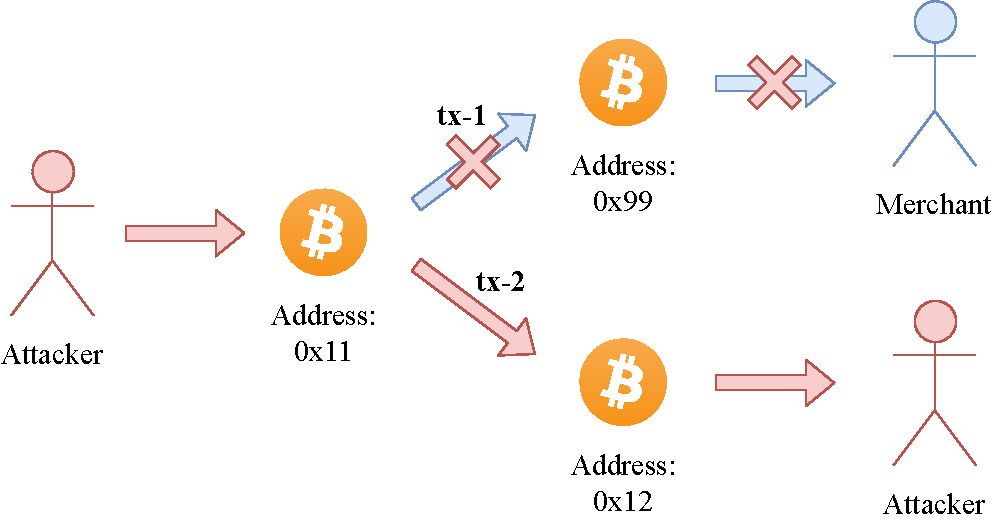
\includegraphics[scale=0.75]{figures/race_attack}
	\vspace*{0.20cm}
	\caption{
		Illustration of the race attack, a variant of double-spending.
		The attacker (in red) owns some bitcoins in the address \texttt{0x11}.
		It submits a transaction \texttt{tx-1} to move the money from its address \texttt{0x11} to the merchant's one \texttt{0x99} (in blue).
		At the same time, it submit to the Bitcoin network a conflicting transaction \texttt{tx-2} to move the the money from \texttt{0x11} to a new address \texttt{0x12} in its control.
		If the network includes \texttt{tx-2} in some block before \texttt{tx-1}, \texttt{tx-1} is rejected, and the money stay control of the attacker.
		The color of the arrows indicates the real flow of bitcoins, after that \texttt{tx-2} is stored in the blockchain and \texttt{tx-1} is rejected.
	}
	\label{fig:race-attack}
\end{figure}

A trivial defense for the merchant is to wait for the transaction \texttt{tx-1} to be stored in the blockchain:
if it is rejected because of any conflicts, the merchant can simply refuse the payment and do not sell the good.
Unfortunately, Bitcoin requires on average \SI{10}{minutes} to confirm a transaction, so this technique can not be always applied.
Bitcoin's developers recommendation is to wait for \num{6} confirmations, i.e. to wait for the block that stored the transaction to be in the longest chain and to have \num{6} following blocks \cite{confirmation}.
Some blocks can be conflicting with each other (if they have the same parent):
only one of them can belong to the longest chain, while the others are said to be ``orphaned'' \cite{orphaned_block} and simply ignored, as illustrated in \cref{fig:orphaned-block}.
Thus, a transaction can be rejected even if it manages to get part of a block, if that block is orphaned.
Waiting for \num{6} confirmations gives a good tradeoff between the time to wait (on average \SI{1}{hour}) and statistical guarantee that the transaction is very unlikely to be rejected later \cite{bitcoin_2009}.

\begin{figure}[h]
	\centering
	\vspace*{0.20cm}
	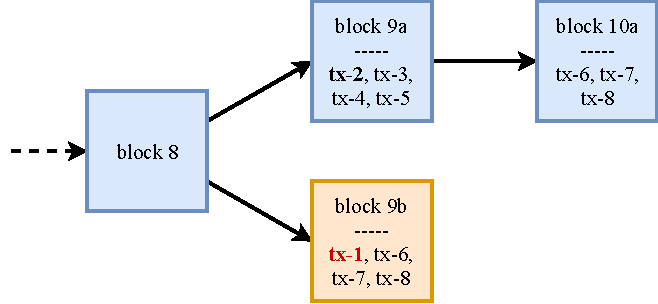
\includegraphics[scale=1.1]{figures/orphaned_block}
	\vspace*{0.20cm}
	\caption{
		Illustration of an orphaned block.
		Blocks \texttt{9a} and \texttt{9b} have the same parent.
		Since \texttt{9a} has a child \texttt{10a}, it is on the longest chain.
		Transactions \texttt{tx-6}, \texttt{tx-7} and \texttt{tx-8} from the orphaned block \texttt{9b} are stored in \texttt{10a};
		\texttt{tx-1} (in red) is in conflict with \texttt{tx-2} and is thus rejected.
	}
	\label{fig:orphaned-block}
\end{figure}

\section{Majority Attack}
51\%
\cite{selfish_mining, selfish_mining_acm}
